%%
\chapter{Funções Reais de Várias Variáveis}
%%
%%%%%%%%%
\section{Derivadas Direcionais e Vetor Gradiente}
%%%%%
Sabemos pela da regra da cadeia que se \(f(x,\; y)\) é diferenciável, então a taxa com que \(f\) varia em
relação a \(t\) ao longo de uma curva diferenciável \(x=g(t)\), \(y = h(t)\) é,
\begin{equation*}
	\frac{df}{dt}=\frac{df}{dx}\,\frac{dx}{dt}+\frac{df}{dy}\,\frac{dy}{dt}
\end{equation*}

Em qualquer ponto \(P_{0}= (x_{0},\;y_{0}) = P_{0}(g(t_{0}),\; h(t_{0}))\), essa equação fornece a taxa de variação de \(f\) em relação a \(t\) e, portanto, depende, entre outras coisas, do sentido do movimento ao longo da curva.

Essa observação e particularmente importante quando a curva é uma reta e \(t\) é o parâmetro de comprimento de arco
ao longo da reta medida de \(P_{0}\) na direção de dado vetor unitário, ou versor, \(u\), pois, nesse caso, \(df/dt\) é a taxa de variação de \(f\) em relação à distância em seu domínio na direção de \(u\). Variando \(u\), encontramos as taxas com que \(f\) varia em relação à distancia quando nos movemos por \(P_{0}\) em direções diferentes. Nesta seção mostremos uma formula para calculá-las e a partir disto podemos encontra fórmulas de equações de planos tangentes e retas normais a superfície $S$ no espaço.

%
\subsection{Derivadas Direcionais no Plano}
%

A seguir desenvolveremos  essa ideia com maior precisão. Suponha que a função \(f(x,\; y)\) seja definida em uma
região \(\Omega\) no plano \(xy\), que \(P_{0}=(x_{0},\; y_{0})\), seja um ponto em \(\Omega\) e que \(u = u_{1}e_{1}
+ u_{2}e_{2}\)  seja um vetor unitário. Então as equações
\begin{equation*}
	x = x_{0}+su_{1}, \quad \text{e}\quad y=y_{0}+su_{2}
\end{equation*}
parametrizam a reta que passa por \(P_{0}\) paralelamente a \(u\). Se o parâmetro \(s\) mede o comprimento de arco de
\(P_{0}\) na direção de \(u\), encontramos a taxa de variação de \(f\) em \(P_{0}\) e na direção de \(u\) calculando
\(df/ds\) em \(P_{0}\).  Veja a Figura~\ref{fig:14-26-thomas}

\begin{defi}[Derivada Direcional]
	A derivada de \(f\)em \(P_{0}(x_{0},\; y_{0})\) na direção do versor \(u = u_{1}e_{1} + u_{2}e_{2}\) é o número
	\begin{equation*}
		(D_{u}f)_{P_{0}}=\left(\frac{df}{ds}\right)_{u,\, P_{0}}=\lim_{s \to 0}
		\dfrac{f(x_{0}+su_{1}, \; y_{0}+su_{2})-f(x_{0},\; y_{0})}{s}
	\end{equation*}
	desde que o limite exista.
\end{defi}

A derivada direcional é denotada também pelo símbolo,
\begin{equation*}
	\left(D_{u}f \right)_{P_{0}} \quad \text{``Derivada de \(f\) em \(P_{0}\) na direção de \(u\)'' }
\end{equation*}

\begin{figure}[!h]
	\centering
	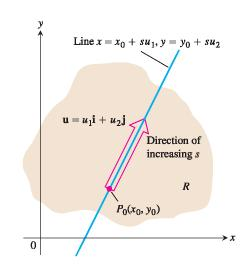
\includegraphics[width=0.4\linewidth]{graphics-14-26-thomas.jpg}
	\caption{A taxa de variação de \(f\) em a direção de \(u\) no ponto \(P_{0}\) é a taxa com que \(f\) varia ao longo desta reta em \(P_{0}\).}
	\label{fig:14-26-thomas}
\end{figure}

A seguir resolveremos um exercício utilizando a definição de derivada direcional,
\begin{exc}
	Encontre a derivada da função,
	\begin{equation*}
		f(x,\; y)=x^{2}+xy
	\end{equation*}
	em \(P_{0}(1,\; 2)\) na direção do vetor unitário \(u = (1/\sqrt{2})\,e_{1}+(1/\sqrt{2})\,e_{2}\)
\end{exc}

\textbf{Solução.}
Calculando o quociente da definição,
\begin{align*}
	\dfrac{f(x_{0}+su_{1}, \; y_{0}+su_{2})-f(x_{0},\; y_{0})}{s} &= \frac{f\left(1+s\cdot \dfrac{1}{\sqrt{2}},\;
		2+s\cdot \dfrac{1}{\sqrt{2}} \right)-f(1,\; 2)}{s} \\
	&=\dfrac{(1+s/\sqrt{2})^{2}+(1+s/\sqrt{2})(2+s/\sqrt{2}))-(1^{2}+1\cdot 2)}{s}\\
	&=\dfrac{\left(1+\dfrac{2s}{\sqrt{2}}+\dfrac{s^{2}}{2}\right)+\left(2+\dfrac{3s}{\sqrt{2}}+\dfrac{s^{2}}{2}\right)-3}{s}\\
	&=\dfrac{s^{2}+\dfrac{5s}{\sqrt{2}}}{s}
\end{align*}

Aplicando limite quando \(s \to 0\) no calculo anterior
\begin{equation*}
	\lim_{s \to 0} \dfrac{s^{2}+\dfrac{5s}{\sqrt{2}}}{s}=\lim_{s \to 0}\left(\dfrac{5}{\sqrt{2}}+s \right)=
	=\left(\frac{5}{\sqrt{2}}+0\right)=\frac{5}{\sqrt{2}}
\end{equation*}

A taxa de variação de \(f(x,\; y) = x^{2} + xy\) em \(P_{0}(1,\; 2)\) na direção de \(u\) é dada por \(D_{u}f((1,\;
2))= 5/\sqrt{2}\).



%
\subsection{Interpretação Geométrica}
%
A equação $z = f(x,\, y)$ representa uma superfície $S$ no espaço. Se $z_{0} = f(x_{0},\, y_{0})$, então o ponto $P(x_{0},\, y_{0},\, z_{0})$ está em
$S$. O plano vertical que passa por $P$ e $P_{0}(x_{0},\, y_{0})$ paralelo a $u$ intercepta $S$ em uma curva $\mathcal{C}$ (Veja
Figura~\ref{fig:14-27-thomas}). A taxa de variação de $f$ na direção de $u$ é a inclinação da tangente a $\mathcal{C}$ em $P$ no sistema destro
formado pelos vetores $u$ e $k$.

Quando $u=i$, a derivada direcional em $P_{0}$ é $\partial_{x}f$ calculada em $(x_{0},\, y_{0})$. Quando $u=j$, a derivada direcional em $P_{0}$ é
$\partial_{y}f$ avaliada em $(x_{0},\, y_{0})$. A derivada direcional generaliza as duas derivadas parciais. Agora podemos pedir a taxa de variação de
$f$ em qualquer direção $u$, não apenas as direções dos versores $i$ e $j$.

\begin{figure}[!h]
	\centering
	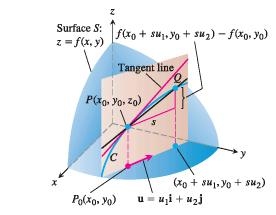
\includegraphics[width=0.65\linewidth]{graphics-14-27-thomas.jpg}
	\caption{A inclinação da curva \(\mathcal{C}\) em \(P_{0}\) é \(\dst{\lim_{p\to Q}}\text{coeficiente angular\,(PQ)}\); esta é a derivada direcional
		\(\left(\dfrac{df}{ds} \right)_{u,\; P_{0}} = (D_{u}f)_{P_{0}}\)}
	\label{fig:14-27-thomas}
\end{figure}

%
\subsection{Cálculos com Derivadas Direcionais}
%

Podemos formular uma segunda definição equivalente,
\begin{defi}[Derivada Direcional]
	Se \(f (x,\; y)\) é uma função de \(x\) e \(y\), e se \(u = u_{1}\,i + u_{2}\, j\) é um vetor unitário, então a derivada direcional de \(f\) na direção de \(u\) em \((x_{0},\; y_{0})\) é denotada por \(D_{u}f (x_{0}, \; y_{0})\) e é definido por
	\begin{equation}\label{eq:2-def}
		D_{u}f(x_{0}, \; y_{0}) =\frac{d}{ds}\bigl[f(x_{0} + su_{1},\;  y_{0} + su_{2})  \bigr]\bigg\vert_{s=0}
	\end{equation}
	desde que esta derivada exista.
\end{defi}


\begin{exc}
	Seja \(f(x,\; y) = xy\). Encontre e interprete \(D_{u}f (1, \; 2) \) para o vetor unitário
	\begin{equation*}
		u = \frac{\sqrt{3}}{2}\, i + \frac{1}{2}\, j.
	\end{equation*}
\end{exc}

\textbf{Solução.}
Conclui-se  a partir  da equação \eqref{eq:2-def} que
\begin{equation*}
	D_{u}f(1,\; 2) =\frac{d}{ds}\left[ f\left(1+\frac{\sqrt{3}}{2}s, \; 2+\frac{1}{2}s \right) \right]\Bigg\vert_{s=0}.
\end{equation*}

Posto que,
\begin{equation*}
	f\left(1+\frac{\sqrt{3}}{2}s, \; 2+\frac{1}{2}s \right)=\left(1+\frac{\sqrt{3}}{2}s \right) \left( 2+\frac{1}{2}s\right)
	=\frac{\sqrt{3}}{4}s^{2}+\left(\frac{1}{2}+\sqrt{3} \right)s + 2,
\end{equation*}
temos
\begin{equation*}
	D_{u}f(1, \; 2) = \frac{d}{ds}\left[ \frac{\sqrt{3}}{4}s^{2}+\left(\frac{1}{2}+\sqrt{3} \right)s + 2 \right]\Bigg\vert_{s=0}=
	\left[ \frac{\sqrt{3}}{2}s+\frac{1}{2} + \sqrt{3}\right]\bigg\vert_{s=0} =\frac{1}{2} + \sqrt{3}.
\end{equation*}

Como \(1/2 + \sqrt{3} \approx 2,23\), concluímos que se movermos uma pequena distância do ponto \((1,\, 2)\) na direção de \(u\), a função
\(f(x,\; y) = xy\) aumentará cerca de \(2,23\) vezes a distância deslocada.

%
\subsection{Cálculos e Gradientes}
%

Agora, vamos desenvolver uma fórmula mais eficiente para calcular a derivada direcional para uma função diferenciável \(f\). Começamos com a reta
\begin{equation}\label{eq:2-thom}
	x=x_{0}+su_{1} \quad \text{e}\quad y=y_{0}+su_{2}
\end{equation}
por \(P_{0}(x_{0},\; y_{0})\), parametrizada pelo comprimento do arco \(s\) aumentando na direção do vetor unitário
\(u =u_{1}e_{1}+u_{2}e_{2}\). Então, utilizando a regra da cadeia
\begin{align}
	(D_{u}f)_{P_{0}} &=\left(\frac{\partial f }{\partial x}\right)_{P_{0}}\frac{dx}{ds}+\left(\frac{\partial f }{\partial
		x} \right)_{P_{0}}\frac{dy}{ds} \notag\\
	&= \left(\frac{\partial f }{\partial x} \right)_{P_{0}}\cdot u_{1}+\left(\frac{\partial f }{\partial y}
	\right)_{P_{0}}\cdot u_{2}\notag\\
	&= \left[\left(\frac{\partial f }{\partial x}\right)_{P_{0}}\,e_{1}+\left(\frac{\partial f }{\partial y}
	\right)_{P_{0}}e_{2}\right]\cdot \left[u_{1}e_{1}+u_{2}e_{2} \right] \label{eq:3-thom}
\end{align}

\begin{defi}[Vetor Gradiente]
	O vetor gradiente (gradiente) de \(f(x,\; y)\) no ponto \( P_{0}(x_{0},\; y_{0}) \) é o vetor
	\begin{equation*}
		\nabla f = \frac{\partial f }{\partial x}\, e_{1}+\frac{\partial f }{\partial y}\, e_{2}=
		\partial_{x}f\, e_{1}+\partial_{y}f\, e_{2}
	\end{equation*}
	obtido por intermédio do calculo de derivadas parciais da função \(f\) no ponto \(P_{0}\).
\end{defi}

A notação \(\nabla f\) e lida tanto como ``\(\rm{grad}\,f\)'' quanto como ``gradiente de \(f\)''. O símbolo
\(\nabla\) isolado é lido como ``nabla''. Outra notação para o gradiente é \( \rm{grad}\, f\), lida da maneira como é
escrita.

A equação \eqref{eq:3-thom} diz que a derivada de \(f\) na direção de \(u\) em \(P_{0}\) é o produto escalar de \(u\)
com o gradiente de \(f\) em \(P_{0}\).

\begin{teo}[Derivada Direcional é um Produto Escalar]
	Se \(f(x,\; y)\) for diferenciável em uma região aberta contendo \(P_{0}(x_{0},\; y_{0})\), então
	\begin{equation}\label{eq:4-thom}
		\left(\frac{df}{ds}\right)_{u,\;P_{0}}=\left(D_{u}f\right)_{P_{0}}=(\nabla f)_{P_{0}}\cdot u
	\end{equation}
	o produto escalar do gradiente de \(f\) em \(P_{0}\) e o vetor \(u\).
\end{teo}


\begin{exc}[Derivada Direcional usando o Gradiente]
	Encontre a derivada de \( f(x,\; y)= xe^{y} +\cos xy\) no ponto \((2,\; 0)\) na direção de \(v = 3\,i -4\,j\),
\end{exc}

\textbf{Solução.}
A direção de \(v\) obtida dividindo-se \(v\) por seu comprimento;
\begin{equation*}
	u=\frac{v}{|v|}=\frac{v}{5}=\frac{3}{5}\, i-\frac{4}{5}\, j
\end{equation*}

As derivadas parciais de \(f\) são contínuas cm todos os pontos e em \((2,\; 0)\) sao dadas por
\begin{align*}
	\partial_{x}f(2,\; 0) & = \left(e^{y}-y\sen(xy)\right)\Big\vert_{(2,\; 0)}=e^{0}-0=1 \\[2ex]
	\partial_{y}f(2,\; 0) & =  \left(xe^{y}-x\sen(xy)\right)\Big\vert_{(2,\; 0)}=2e^{0}-2\cdot 0=2
\end{align*}

O gradiente de \(f\) em \((2,\; 0)\) é
\begin{equation*}
	\nabla f\Big\vert_{(2,\; 0)}=\partial_{x}f(2,\; 0)\, i +\partial_{y}f(2,\; 0)\, j = i+2\, j
\end{equation*}
Veja a Figura~\ref{fig:14-28-thomas}

A derivada de \(f\) em \((2,\; 0)\) na direção de \( v \) é, portanto,
\begin{equation*}
	(D_{u}f)_{(2,\;0)}=\nabla f\Big|_{(2,\; 0)}\cdot u =(i+2\,j)\cdot\left(\frac{3}{5}\, i-\frac{4}{5}\, j \right)=\frac{3}{5}-\frac{8}{5}=-1
\end{equation*}
e isso conclui o exercício. \hfill $\lozenge$

\begin{figure}[!h]
	\centering
	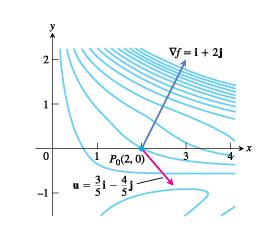
\includegraphics[width=0.45\linewidth]{graphics-14-28-thomas.jpg}
	\caption{A taxa com que $f$ varia na direção de $u$ é \(\nabla f\cdot u=-1$}
	\label{fig:14-28-thomas}
\end{figure}


%
\subsection{Propriedades da Derivada Direcional}
%

O cálculo do produto escalar na formula
\begin{equation*}
	D_{u}f = \nabla f\cdot u = |\nabla f||u|\cos \theta =|\nabla f| \cos \theta
\end{equation*}
onde \(\theta\) é o ângulo entre os vetores \(u\) e \(\nabla f\) revela-nos as propriedades a seguir.

\begin{figure}[!h]
	\centering
	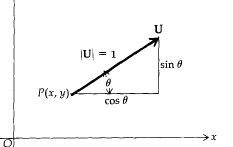
\includegraphics[width=0.3\linewidth]{calculus-directions-leithold.png}
	\caption{\(U\) é o vetor unitário \(\cos \theta \, i + \sen \theta\, j\) }\label{fig:17-7-1}
\end{figure}

\begin{figure}[!h]
	\centering
	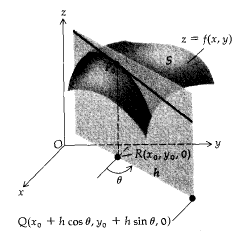
\includegraphics[width=0.3\linewidth]{calculus-directions-leithold01.png}
	\caption{Definição de derivada direcional com vetor unitário \(u=\cos\theta\,i +\sen \theta\, j\)}
	\label{fig:17-7-2}
\end{figure}

\begin{itemize}
	\item A função \(f\) aumenta mais rapidamente quando \(\cos \theta = 1\) ou quando \(u\) é a direção de \(\nabla f\).
	Isto é, a cada ponto \(P\) no seu domínio, \(\nabla\, f\) cresce mais rapidamente na direção  e no sentido do vetor gradiente \(\nabla f \) em \(P\). A derivada nessa direção é
	\begin{equation*}
		D_{u}f=|\nabla\, f|\cos 0 = |\nabla\, f|.
	\end{equation*}
	
	\item De maneira similar, \(f\) decresce mais rapidamente na direção e no sentido de \(-\nabla f \). A derivada nessa direção é
	\begin{equation*}
		D_{u}f=|\nabla f|\cos \pi = -|\nabla f|.
	\end{equation*}
	
	\item Qualquer direção \(u\) ortogonal ao gradiente \(\nabla\, f \neq 0\) é uma direção de variação zero em \(f\) porque \(\theta\) é então igual a \( \pi/2\) e
	\begin{equation*}
		D_{u}f=|\nabla\, f|\cos\left(\frac{\pi}{2} \right) = |\nabla\, f|\cdot 0= 0.
	\end{equation*}
\end{itemize}

Como veremos mais à frente, essas propriedades são verdadeiras tanto em três dimensões como em duas.
\begin{exc}[Direções de Variação Máxima, Mínima e Zero]
	Encontre as direções nas quais
	\begin{equation*}
		f(x,\; y) = \frac{x^{2}}{2} + \frac{y^{2}}{2}.
	\end{equation*}
	\begin{tasks}[label=(\alph*),item-indent=3em,label-width=4ex,ref=(\alph*)](2)
		\task Cresce mais rapidamente no ponto \((1,\; 1)\);
		\task Decresce mais rapidamente em \((1,\; 1)\);
		\task! Quais são as direções de variação zero de \(f\) em \((1,\; 1)\)?
	\end{tasks}
\end{exc}

\textbf{Solução.}

(a) A função aumenta mais rapidamente na direção e no sentido de \(\nabla f\) em \( (1,\; 1)\). O gradiente nesse ponto é
\begin{equation*}
	(\nabla f)_{(1,\; 1)}=(x\, i + y\, j)\Big\vert_{(1,\; 1)}=i+j.
\end{equation*}

Sua direção ou versor é,
\begin{equation*}
	u=\dfrac{(\nabla f)_{(1,\; 1)}}{|(\nabla f)_{(1,\; 1)}|} =\dfrac{i+j}{|i+j|}=\dfrac{i+j}{\sqrt{(1)^{2}+(1)^{2}}}=\frac{1}{\sqrt{2}}\, i + \frac{1}{\sqrt{2}}\, j
\end{equation*}

(b) A função decresce mais rapidamente na direção e no sentido de \(-\nabla f\) em \((1,\; 1)\), e sua direção ou versor é,
\begin{equation*}
	-u =-\dfrac{(\nabla f)_{(1,\; 1)}}{|(\nabla f)_{(1,\; 1)}|} =-\frac{1}{\sqrt{2}}\, i - \frac{1}{\sqrt{2}}\, j
\end{equation*}

(c) As direções de variação zero em \((1,\; 1)\) são as direções ortogonais a \(\nabla f\),
\begin{equation*}
	n=-\frac{1}{\sqrt{2}}\, i + \frac{1}{\sqrt{2}}\, j \quad \text{ e }\quad -n=\frac{1}{\sqrt{2}}\, i - \frac{1}{\sqrt{2}}\, j
\end{equation*}
Veja a Figura~\ref{fig:14-29-thomas}.

\begin{figure}[!h]
	\centering
	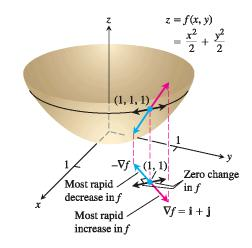
\includegraphics[width=0.4\linewidth]{graphics-14-29-thomas.jpg}
	\caption{A direção em que $f(x,\, y)$ aumenta mais rapidamente em \((1,\; 1)\) é
		a direção de \((\nabla f)_{(1,\, 1)}=i+j\). Corresponde à direção e ao sentido de subida mais íngreme na superfície em \((1,\, 1,\, 1)\)}
	\label{fig:14-29-thomas}
\end{figure}



%
\subsection*{Gradientes e Reta Tangente a Curvas de Nível}
%

Se uma função diferenciável \(f(x,\; y)\) tiver um valor constante \(C\) ao longo de uma curva lisa
\(\alpha(t) = g(t)\,i + h(t)\, j)\) (fazendo da curva uma curva de nível de \(f\)), então \(f(g(t),\; h(t))=C\).

Derivar ambos os lados dessa equação em relação a \(t\), usando a regra da cadeia leva às equações
\begin{equation*}
	\frac{d}{dt}f(g(t),\; h(t))  =\frac{d}{dt}\, C,
\end{equation*}
e pela regra da cadeia,
\begin{equation*}
	\frac{\partial\, f}{\partial x}\frac{dg}{dt}\, i + \frac{\partial\, f}{\partial y}\frac{dh}{dt}\, j  = 0.
\end{equation*}

Portanto,
\begin{equation}\label{eq:5-thom}
	\left(\frac{\partial f}{\partial x}\, i+\frac{\partial f}{\partial y}\, j \right)\cdot \left(\frac{dg}{dt}\, i + \frac{dh}{dt}\, j \right) = 0.
\end{equation}

A equação \eqref{eq:5-thom} diz que \(\nabla\, f\) é normal ao vetor tangente \(\alpha'(t)\), portanto é normal à curva.


Em todo ponto \((x_{0},\; y_{0})\) no domínio de uma função diferenciável \(f(x,\; y)\) o gradiente d e \(f\) normal à curva de nível que passa por \((x_{0},\; y_{0})\).

A equação \eqref{eq:5-thom} confirma nossa observação dc que os córregos correm perpendicularmente às curvas de nível em mapas topográficos.

Como o córrego deve alcançar seu destino da maneira mais rápida, deve correr na direção oposta á dos gradientes, devido a Propriedade 2 da derivada direcional. A equação \eqref{eq:5-thom} nos diz que essas direções são perpendiculares às curvas de nível.

Essa observação também nos permite encontrar equações para retas tangentes às curvas de nível. Elas são as retas normais aos gradientes. A reta que passa por um ponto \(P_{0}(x_{0},\;y_{0})\) normal a um vetor \(N = A\,i +B\,j\) tem a equação
\begin{equation*}
	A(x-x_{0})+B(y-y_{0})=0
\end{equation*}

Se \(N\) é o gradiente
\begin{equation*}
	(\nabla f)_{P_{0}}= \partial_{x}f(P_{0})\, i +\partial_{y}f(P_{0})\, j
\end{equation*}
a equação torna-se
\begin{equation}\label{eq:6-thom}
	\partial_{x}f(x_{0},\; y_{0})(x-x_{0})+\partial_{y}f(x_{0},\; y_{0})(y-y_{0})=0
\end{equation}

\begin{exc}[Reta Tangente a uma Elipse]
	Encontre uma equação para a tangente à elipse
	\begin{equation*}
		\frac{x^{2}}{4}+y^{2} =2
	\end{equation*}
	no ponto \((-2, \; 1)\).
\end{exc}

\solo
A elipse é uma curva de nível da função
\begin{equation*}
	f(x,\; y) = \frac{x^{2}}{4}+y^{2}
\end{equation*}

O gradiente de \(f\) em \((-2,\;  1)\)  é,
\begin{equation*}
	\nabla f\Big\vert_{(-2,\; 1)}=\left(\frac{x}{2}\, i + 2y\, j \right)\Bigg\vert_{(-2,\; 1)}= -i+2\, j
\end{equation*}

A tangente é a reta
\begin{equation*}
	(-1)(x+2)+(2)(y-1)=0
\end{equation*}

Assim
\begin{equation*}
	x-2y = -4
\end{equation*}

Se soubermos os gradientes de duas funções \(f\) e \(g\), automaticamente saberemos os gradientes de sua soma e diferença, de seu produto e quociente e da multiplicação por uma constante.

O estudante deverá justificar essas propriedades nas listas de Exercícios Propostos. Observe que elas tem a mesma forma que as propriedades correspondentes para derivadas de funções de uma variável

%
\subsection{Propriedades Algébricas do Vetor Gradiente}
%
Multiplicação por constante,
\begin{equation*}
	\nabla ( k\, f ) = k\, \nabla f \quad \text{para qualquer número}\quad  k.
\end{equation*}

Regra da Adição
\begin{equation*}
	\nabla( f+g) = \nabla f + \nabla g
\end{equation*}

Regra do produto
\begin{equation*}
	\nabla (fg) = f\, \nabla g + g\nabla\, f
\end{equation*}

Regra do Quociente
\begin{equation*}
	\nabla \left(\frac{f}{g} \right) = \frac{g\nabla f - f \nabla g}{g^{2}}
\end{equation*}

\bigskip
\begin{exc}
	Verificar as propriedades do gradiente utilizando as seguintes funções escalares,
	\begin{equation*}
		f(x,\, y)=x-y \quad \text{e} \quad g(x,\; y)=3y
	\end{equation*}
\end{exc}

\solo
Calculamos o gradiente de cada função rela de duas variáveis,
\begin{equation*}
	\nabla f = i-j\quad \text{ e } \quad \nabla g =3\,j.
\end{equation*}

Para uma constante qualquer \( k =2\),
\begin{equation*}
	\nabla(2f) = \nabla (2x-2y)=i+ 2\,j=2\,\nabla f
\end{equation*}

O gradiente da soma,
\begin{equation*}
	\nabla(f+g)= \nabla(x+2y) = i + 2\, j=\nabla f + \nabla g
\end{equation*}

O gradiente da soma,
\begin{equation*}
	\nabla(f-g)= \nabla(x-4y) = i -4\, j=\nabla f - \nabla g
\end{equation*}

O gradiente do produto,
\begin{align*}
	\nabla(f\, g) &= \nabla (3xy-3y^{2}) = 3y\, i +(3x-6y)\, j \\[2ex]
	&= 3y(i-j)+3y\,j+(3x-6y)\,j\\[2ex]
	&= 3y(i-j)+(3x-3y)\,j\\[2ex]
	&= 3y(i-j)+(x-y)3\,j = g\nabla f+ f\, \nabla g
\end{align*}

O gradiente do quociente
\begin{align*}
	\nabla\left(\frac{f}{g}\right) & = \nabla \left(\frac{x-y}{3y} \right)= \nabla \left(\frac{x}{3y}-\frac{1}{3}\right) \\
	& = \frac{1}{3y}\, i -\frac{x}{3y^{2}}\,j\\
	&=\dfrac{3y\,i-3x\,j}{9y^{2}}=\frac{3y(i-j)-(3x-3y)\, j}{9y^{2}}\\
	&=\frac{3y(i-j)-(x-y)3j}{9y^{2}}=\frac{g\nabla f-f\nabla g}{g^{2}}.
\end{align*}

%
\subsection{Funções Reais de Três Variáveis}
%
Para uma função diferenciável \(f(x,\; y,\; z)\) e um vetor unitário \(u = u_{1}\,i +u_{2}\,j+u_{1}\,k\) no espaço, temos
\begin{equation*}
	\nabla f = \frac{\partial f}{\partial x}\, e_{1}+\frac{\partial f}{\partial y}\, e_{2} +
	\frac{\partial f}{\partial z}\, e_{3}
\end{equation*}
e
\begin{equation*}
	D_{u}f= \nabla f \cdot u =\frac{\partial f}{\partial x}u_{1}+\frac{\partial f}{\partial x}u_{2}
	+\frac{\partial f}{\partial z}u_{3}
\end{equation*}

A derivada direcional pode ser escrita novamente na forma
\begin{equation*}
	D_{u}f= \nabla f \cdot u =|\nabla f||u| \cos \theta= |\nabla f|\cos \theta
\end{equation*}
assim as propriedades relacionadas anteriormente para funções de duas variáveis continuam valendo. Em qualquer ponto
dado, \(f\) aumenta mais rapidamente na direção de \(\nabla f\) e decresce mais rapidamente na direção de \(-\nabla
f\). Em qualquer direção ortogonal a \(\nabla f\) a derivada é zero,

\begin{exc}[Direções de variação máxima, mínima e zero]
	Resolva em detalhes as seguintes questões
	\begin{enumerate}
		\item[\rm{(a)}] Encontre a derivada de \(f(x,\; y,\; z) = x^{3}-xy^{2}-z\) em \(P_{0}(1,\; 1,\; 0)\) na direção de \(v = 2i
		-3j + 6\, k\).
		\item[\rm{(b)}] Em que direções \(f\) varia mais rapidamente em \(P_{0}\) e quais são as taxas de variação nessas direções?
	\end{enumerate}
\end{exc}

\solo
A direção de \(v\) é obtida dividindo-se \(v\) pelo seu comprimento,
\begin{equation*}
	|v|=\sqrt{(2)^{2}+(-3)^{2}+(6)^{2}}=\sqrt{49}=7
\end{equation*}
logo,
\begin{equation*}
	u=\frac{v}{|v|}=\frac{2}{7}\, i -\frac{3}{7}\, j+\frac{6}{7}\,k
\end{equation*}

As derivadas parciais de \(f\) em \(P_{0}\), são
\begin{equation*}
	\partial_{x}f=(3x^{2}-y^{2})\Big\vert_{(1,\;1, \; 0)}=2, \quad \partial_{y}f=-2xy\Big\vert_{(1,\;1, \; 0)}=-2, \quad \partial_{z}f=-1\Big\vert_{(1,\;1, \; 0)}=-1
\end{equation*}

O gradiente de \(f\) em \(P_{0}\) é
\begin{equation*}
	\nabla f\Big\vert_{(1,\; 1, \; 0)}=2\,i-2\,j-k.
\end{equation*}

A derivada direcional de \(f\) em \(P_{0}\) na direção de \(v\) é, portanto,
\begin{align*}
	(D_{u}f)_{(1,\;1,\; 0)} & = \nabla f\Big\vert_{(1,\; 1, \; 0)}\cdot u =(2i-2j-k)\cdot \left(\frac{2}{7}i-\frac{3}{7}\,j+\frac{6}{7}\, k \right) \\[2ex]
	&=\frac{4}{7}+\frac{6}{7}-\frac{6}{7}=\frac{4}{7}.
\end{align*}

(b) A função cresce mais rapidamente na direção de \( \nabla f = 2i - 2j-k\) e decresce mais rapidamente na direção
do vetor \(-\nabla f\). As taxas de variação nas direções são, respectivamente,
\begin{equation*}
	|\nabla f|=\sqrt{(2)^{2}+(-2)^{2}+(-1)^{2}}=\sqrt{9}=3 \quad \text{e} \quad -|\nabla f| =-3.
\end{equation*}

%
\section{Campos Vetoriais}
%

Um \textsf{campo vetorial} em \(\mathbb{R}^{n}\) é uma função \(\mathbf{F} \colon  A \subset \mathbb{R}^{n} \to  \mathbb{R}^{n}\) que atribui a cada
ponto \(\mathbf{x}\) em seu domínio \(A\) um vetor \(\mathbf{F}(\mathbf{x})\).  Se \(n = 2\), a função \(F\) é chamada de \textsc{campo vetorial no
	plano} e se \(n = 3\), a função \(\mathbf{F}\) é um \textsc{campo vetorial no espaço}.

O campo \(\mathbf{F}\) figura como anexado uma seta em cada ponto (Veja a Figura~\ref{fig:4-3-1}).
\begin{figure}[h]
	\centering
	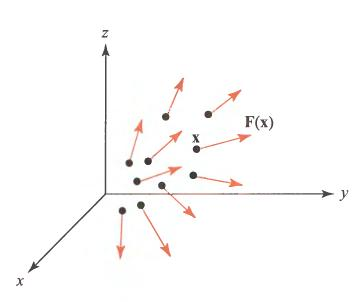
\includegraphics[width=3.0in]{figura-calculus-marsden431-col.jpg}
	\caption{Um campo vetorial \(\mathbf{F}\) atribui um vetor \(\mathbf{F}(\mathbf{x})\) a cada ponto \(\mathbf{x}\) de seu domínio }\label{fig:4-3-1}
\end{figure}

Em contraste, uma função \(f \colon  A \subset  \mathbb{R}^{n} \to \mathbb{R}\) que atribui um número a cada ponto de seu domínio é um \textsc{campo
	escalar}.

Um campo vetorial \(\mathbf{F}(x,\, y,\, z) \) em \(\mathbb{R}^{3} \)  tem \textsf{três campos escalares} componentes \(F_{1}\),  \(F_{2}\) e \(F_{3}\) de modo
que
\begin{equation*}
	\mathbf{F}(x,\, y,\, z) =\left(F_{1} (x, \, y,\,  z),\; F_{2} (x, \, y,\,  z),\;  F_{3} (x,\,  y,\,  z)\right).
\end{equation*}

Se cada uma das componentes \(F_{1}\), \(F_{2}\) e \(F_{3}\) é uma função de classe \(C^{k}\), dizemos que o campo vetorial \(\mathbf{F}\) é da classe \(C^{k}\), os campos vetoriais serão assumidos no que segue como sendo pelo menos da classe \(C^{1}\), a menos que indicado de outra forma.

Em muitas aplicações, \(\mathbf{F}(\mathbf{x})\) representa uma grandeza vetorial física (força, velocidade, etc.) associada à posição \(\mathbf{x}\).

Visualizamos campos vetoriais traçando a seta que representa $\mathbf{F}(x,\; y)$ no ponto $(x,\; y)$ ou $\mathbf{F}(x,\; y,\; z)$ em cada ponto
$(x,\; y,\; z)$.

Obviamente, não podemos fazer isso para todos os pontos, então fazemos isso para alguns pontos representativos. Também podemos usar software
matemático para plotar um campo vetorial. O comando em cada software para plotar um campo vetorial depende se é um campo vetorial em $\mathbb{R}^{2}$
ou $\mathbb{R}^{3}$.

%
\section{Operações de Divergência e Rotacional}
%

Para cada uma das operações de divergência e rotacional, faremos uso do operador ``del'', definido por
\begin{equation*}
	\nabla = i\, \partial_{x}+j\, \partial_{y}+k\, \partial_{z}
\end{equation*}

Para funções de uma variável, a obtenção de uma derivada pode ser considerada uma operação ou processo; isto é, dada uma função \(y = f (x)\), sua derivada é o resultado da operação em \(y\) pelo operador derivação \(D=d/dx\). Da mesma forma, podemos escrever o gradiente de \(f\) como
\begin{equation*}
	\nabla f =\left(i\, \partial_{x}+j\, \partial_{y}\right)\, f = i\, \partial_{x} f+j\, \partial_{y} f,
\end{equation*}
para funções de duas variáveis, e
\begin{equation*}
	\nabla f =\left( i\, \partial_{x}+j\, \partial_{y}+k\, \partial_{z}\right)\, f= i\, \partial_{x} f+j\, \partial_{y}f+k\, \partial_{z} f
\end{equation*}
para três variáveis. Em termos operacionais, \textsf{o gradiente de} \(f\) é obtido tomando o operador \(\nabla\) e aplicando-o para o \textsf{campo
	escalar} \(f\).

%
\subsection*{Definição da Divergência}
%

Definimos a divergência de um campo vetorial \(\mathbf{F}\) tomando o produto escalar do operador  \(\nabla\) com o campo vetorial \(\mathbf{F}\).

\begin{defi}[Divergência]
	Se \(\mathbf{F} =F_{1}\, i + F_{2}\, j + F_{3}\, k\) campo vetorial em $\mathbb{R}^{3}$, a divergência de \( \mathbf{F}\) é o campo escalar
	\begin{equation*}
		\mathrm{div}\, \mathbf{F}= \nabla\cdot \mathbf{F} = \partial_{x}F_{1}+ \partial_{y}F_{2}+\partial_{z}F_{3}
	\end{equation*}
\end{defi}

Da mesma forma, se \(\mathbf{F} = (F_{1},\ldots, F_{n})\) é um campo vetorial em \(\mathbb{R}^{n}\), sua divergência é
\begin{equation*}
	\mathrm{div}\, \mathbf{F} = \nabla \cdot F= \sum_{i=1}^{n}\partial_{x_{i}}F_{i}=\partial_{x_{1}}F_{1}+ \partial_{x_{2}}F_{2}+\cdots+\partial_{x_{n}}F_{n}
\end{equation*}

\begin{exc}
	Calcular a divergência do seguinte campo vetorial
	\begin{equation*}
		\mathbf{F}(x,\, y,\, z) = x^{2}y\,i + z\, j + xyz\, k.
	\end{equation*}
	em $\mathbb{R}^{3}$.
\end{exc}

\solo
Ao aplicar a definição de divergência devemos calcular primeiro as derivadas parciais na direção se sentido dos versores ou vetores
unitários canônicos, isto é,
\begin{equation*}
	\partial_{x}F_{1}(x,\, y, \, z)= 2xy ;  \quad \partial_{y}F_{2}(x,\, y, \, z)=0 ; \quad \partial_{z}F_{3}(x,\, y, \, z)=xy
\end{equation*}

Logo obtemos,
\begin{equation*}
	\mathrm{div}\, \mathbf{F} = \nabla \cdot \mathbf{F} = \partial_{x}F_{1}+\partial_{y}F_{2}+\partial_{z}F_{3} =2xy+0+xy=3xy
\end{equation*}
que é o \textsf{campo escalar divergência}. \hfill $\lozenge$

\bigskip
A divergência tem uma importante interpretação física. Se imaginarmos \(\mathbf{F}\) para ser o campo de velocidade de um gás (ou um fluido), então
\(\mathrm{div}\; \mathbf{F}\) representa a \textit{taxa de expansão por unidade de volume sob o fluxo do gás} (ou fluido). Se \(\mathrm{div}\; \mathbf{F} < 0\), o gás
(ou fluido) está comprimindo. Para um campo vetorial \(\mathbf{F}(x,\; y) = F_{1}\,i + F_{2}\, j\) no plano, a divergência,
\begin{equation*}
	\nabla\cdot \mathbf{F} = \partial_{x}F_{1}+\partial_{y}F_{2}
\end{equation*}
mede a taxa de expansão da área.

Esta interpretação é explicada graficamente, como segue. Escolha uma pequena região \(W\) com um ponto \(\mathbf{x}_{0}\). Para cada ponto
\(\mathbf{x}\) em \(W\), defina \(\mathbf{x}(t)\) ser a linha de fluxo emanando de \(\mathbf{x}\). O conjunto de pontos \(\mathbf{x}(t)\) descreve
como o conjunto \(W\) flui após o tempo \(t\) (veja a Figura~\ref{fig:4-4-1}).

\begin{figure}[H]
	\centering
	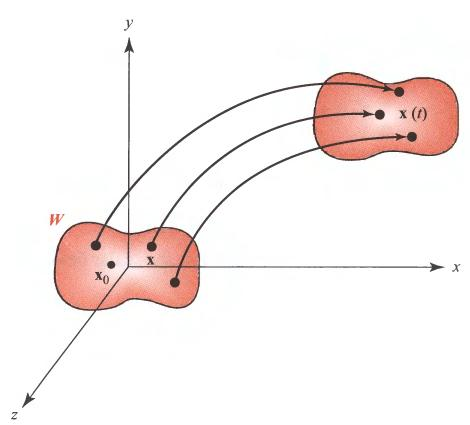
\includegraphics[width=0.4\linewidth]{figura-marsden441.jpg}
	\caption{ Uma região \(W\) fluindo ao longo das linhas de fluxo de um campo vetorial.}
	\label{fig:4-4-1}
\end{figure}

Denota-se para a região que resulta depois que o tempo \(t\) decorreu com \(W (t)\), e seja \(V(t)\)  seu volume (ou área em duas
dimensões). Então a \textit{taxa relativa de mudança de volume} é a divergência; mais precisamente,
\begin{equation*}
	\dfrac{1}{V(0)}\dfrac{d}{dt}V(t)\Bigg{\vert}_{t=0}\approx \mathrm{div\,}\mathbf{F}(0)
\end{equation*}
com a aproximação sendo mais exata quando \(W\) encolhe cada vez mais para \(\mathbf{x}_{0}\).

\begin{exc}
	Considere o campo vetorial num avião dado por \(\mathbf{V}(x,\; y) = x\, i\). Relacionar o sinal da divergência de \(\mathbf{V}\) com a taxa de mudança de
	áreas sob o fluxo.
\end{exc}

\solo Pensamos no campo vetorial \(\mathbf{V}\)  como o campo de velocidade de um fluido no plano. O campo vetorial \(\mathbf{V}\) aponta para a
direita quando \(x>0\) e à esquerda se \(x<0\), como vemos na Figura~\ref{fig:4-4-2}.

\begin{figure}[H]
	\centering
	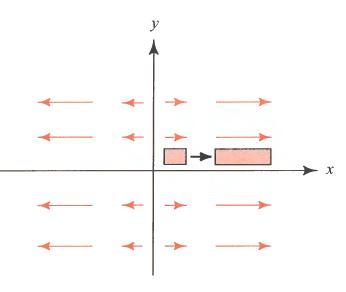
\includegraphics[width=0.5\linewidth]{figura-marsden442}
	\caption{O fluido está se expandindo.}
	\label{fig:4-4-2}
\end{figure}

O comprimento de \(\mathbf{V}\) fica mais curto em direção à origem. Como o fluido se move, ele se expande (a área do retângulo sombreado
aumenta), então esperamos \(\mathrm{div}\; \mathbf{V} > 0\). De fato, efetuando-se o calculo do campo escala divergência, valida-se a nossa conjectura,
isto é,
\begin{equation*}
	\mathrm{div}\; \mathbf{V} =\nabla\cdot \mathbf{V} = \partial_{x}V_{1}(x,\; y)+\partial_{y}V_{2}(x,\; y)=1+0=1 > 0
\end{equation*}

\begin{exc}
	As linhas de fluxo do campo vetorial \(\mathbf{F} = x\, i + y\, j\) são linhas retas direcionadas para longe da origem, relacionar o sinal do
	campo escalar divergência  com a taxa de expansão se as linhas de fluxo fossem de um fluído.
\end{exc}

\solo
Como linhas de fluxo são de um fluido, observamos que o fluido está se expandindo, pois se move afastando-se da origem, de modo que
\(\mathrm{div}\; \mathbf{F}\) deve ser positivo. Na verdade, calculando o divergente usando a definição obtemos,
\begin{equation*}
	\mathrm{div}\; \mathbf{F} =\nabla \cdot \mathbf{F}= \partial_{x}F_{1}(x,\; y)+\partial_{y}F_{2}(x,\; y)=1+1=2>0,
\end{equation*}
o que confirma a nossa afirmação. Veja a Figura~\ref{fig:4-4-3}.

\begin{figure}[H]
	\centering
	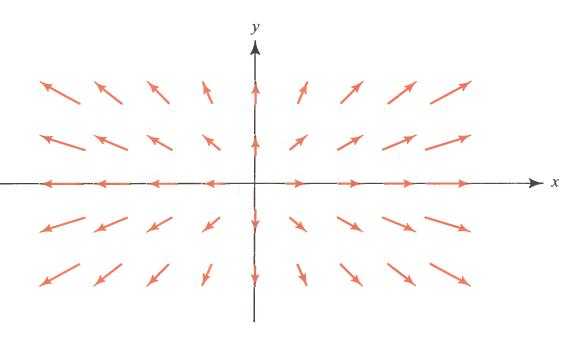
\includegraphics[width=0.5\linewidth]{figura-marsden443}
	\caption{O campo vetorial \(\mathbf{F}(x,\; y) = x\, i + y\, j\)}
	\label{fig:4-4-3}
\end{figure}

%
\section{O Rotacional de um Campo Vetorial}
%
Para calcular o rotacional, a segunda operação básica realizada em campos vetoriais, aplicamos o produto cruz do operador \(\nabla\) com o campo vetorial \(\mathbf{F}\).

\begin{defi}[Rotacional]
	Se \(\mathbf{F} = F_{1}\, i + F_{2}\, j + F_{3}\, k\) é um campo vetorial em $\mathbb{R}^{3}$,  o rotacional de \(\mathbf{F}\) é o campo vetorial em $\mathbb{R}^{3}$ dado por,
	\begin{align*}
		\nabla\times F &= \left(\partial_{y}F_{3}-\partial_{z}F_{2}\right)\,i +\left(\partial_{z}F_{1}-\partial_{x}F_{3}\right)\, j
		+\left(\partial_{x}F_{2}-\partial_{y}F_{1} \right)\, k \\[3ex]
		&=\left|\begin{array}[c]{ccc}
			i& j & k\\
			\partial_{x} & \partial_{y} & \partial_{z}\\
			F_{1} & F_{2} & F_{3}		
		\end{array}
		\right|.
	\end{align*}
\end{defi}

Se escrevermos o campo vetorial por \(\mathbf{F} = P\,i + Q\,j + R\,k\) em $\mathbb{R}^{3}$, que é notação alternativa, a mesma fórmula para o rotacional será,
\begin{align*}
	\nabla\times F &= \left(\partial_{y}R-\partial_{z}Q\right)\,i +\left(\partial_{z}P-\partial_{x}R\right)\, j
	+\left(\partial_{x}Q-\partial_{y}P \right)\, k \\[3ex]
	&=\left|\begin{array}[c]{ccc}
		i& j & k\\
		\partial_{x} & \partial_{y} & \partial_{z}\\
		P & Q & R		
	\end{array}
	\right|.	
\end{align*}

A seguir resolvemos alguns exercícios para fixar e reforçar algumas ideias e conceitos.
\begin{exc}
	Considere o campo vetorial em $\mathbb{R}^{3}$, \(\mathbf{F}(x,\; y,\; z) = x\, i + xy\, j + k\). Encontre o rotacional \(\nabla \times \mathbf{F}\).
\end{exc}

\solo
Usamos a fórmula do rotacional anterior,
\begin{equation*}
	\nabla \times \mathbf{F} =
	\left|\begin{array}[c]{ccc}
		i & j & k\\
		\partial_{x} & \partial_{y} & \partial_{z}\\
		x & xy & 1		
	\end{array}
	\right|	= (0-0)\, i - (0-0)\, j + (y-0)\, k= y\, k.
\end{equation*}

Assim,
\begin{equation*}
	\nabla \times \mathbf{F} = y\, k.
\end{equation*}
é o rotacional procurado. \hfill $\lozenge$


\begin{exc}
	Encontre o rotacional do campo vetorial  \(\mathbf{F}=xy\, i -\sen z\, j + k\) em $\mathbb{R}^{3}$.
\end{exc}

\solo
Aplicando a definição de rotacional ao campo vetorial,
\begin{equation*}
	\nabla \times \mathbf{F} =
	\left|\begin{array}[c]{ccc}
		i & j & k\\
		\partial_{x} & \partial_{y} & \partial_{z}\\
		xy & -\sen z & 1		
	\end{array}
	\right|	= \left|\begin{array}{cc}
		\partial_{y} & \partial_{z}\\
		-\sen z & 1
	\end{array} \right|\, i - \left|\begin{array}{cc}
		\partial_{x} & \partial_{z}\\
		xy & 1
	\end{array} \right|\, j + \left|\begin{array}{cc}
		\partial_{x} & \partial_{y}\\
		xy & -\sen z
	\end{array} \right|\, k
\end{equation*}

Portanto,
\begin{equation*}
	\nabla\times \mathbf{F} = \cos z\, i -x\, k,
\end{equation*}
é a resposta do rotacional procurado. \hfill $\lozenge$

Ao contrário da divergência, que pode ser definida em \(\mathbb{R}^{n}\) para qualquer \(n\), definimos o rotacional apenas no espaço
tridimensional (ou para campos vetoriais planares, em relação ao terceiro componente como zero).

O significado físico do rotacional será discutido no Capítulo posterior, quando estudarmos o teorema de Stokes. No entanto, podemos agora considerar
uma situação específica, em que o \textsf{rotacional} está associada a \textsf{rotações}.

\bigskip
A seguinte identidade é uma relação básica entre o gradiente e o rotacional, que deve ser comparada com o fato de que para qualquer vetor $\mathbf{v}$, temos que seu produto cruz resulta em  \(\mathbf{v} \times \mathbf{v} = 0\).

%
\subsection*{Rotacional de um Gradiente}
%
Para quaisquer campo escalar $f$ de classe $C^{2}$
\begin{equation*}
	\mathrm{rot}\; \nabla f = \nabla \times (\nabla f)= \mathbf{0}.
\end{equation*}

Ou seja, o \textsf{rotacional} de qualquer campo gradiente é o vetor zero.

\prova
Pela definição $\nabla f=(\partial_{x}f, \; \partial_{y}f, \; \partial_{z}f )$, assim outra vez pela definição de rotacional,
\begin{align*}
	\mathrm{rot}\; \nabla f =\nabla \times \nabla f &=
	\begin{vmatrix}
		i & j & k \\
		\partial_{x} & \partial_{y} & \partial_{z} \\
		\partial_{x}f & \partial_{y}f & \partial_{z}f
	\end{vmatrix}\\[2ex]
	&=\left(\partial_{yz}^{2}f-\partial_{zy}^{2}f \right)\,i+\left(\partial_{zx}^{2}f-\partial_{xz}^{2}f \right)\,j+\left(\partial_{xy}^{2}f
	-\partial_{yx}^{2}f \right)\,k=\mathbf{0}.
\end{align*}

Cada componente é zero devido à igualdade das derivadas parciais mistas. \hfill $\square$

\begin{exc}
	Seja o campo vetorial $\mathbf{V}(x,\; y, \; z)=y\, i-x\, j$ em $\mathbb{R}^{3}$. Mostre que $\mathbf{V}$ não é um campo gradiente
\end{exc}

\solo
Se o campo vetorial $\mathbf{V}$ fosse um campo gradiente, então ele satisfaria $\nabla\times \mathbf{V} = \mathbf{0}$ pela afirmação mostrada anteriormente. Mas o rotacional de $\mathbf{V}$ é,
\begin{equation*}
	\mathrm{rot}\, \mathbf{V} = \nabla\times V=
	\begin{vmatrix}
		i & j & k \\
		\partial_{x} & \partial_{y} & \partial_{z} \\
		y & -x & 0
	\end{vmatrix}= -2\,k  \neq \mathbf{0}
\end{equation*}
que é  contraditório, logo $\mathbf{V}$ não e um campo gradiente. \hfill $\lozenge$

\bigskip
Existe uma operação em campos vetoriais no plano que está intimamente relacionada ao rotacional. Se $\mathbf{F} = P(x,\; y)\,i + Q(x,\; y)\,j$ é um campo
vetorial no plano, ele também pode ser considerado como um campo vetorial no espaço para o qual o componente $k$ é zero e os outros dois componentes são independentes de $z$. O rotacional de $F$ então se reduz a
\begin{equation*}
	\nabla \times \mathbf{F} = \Bigl(\partial_{x}\, Q(x,\; y) -\partial_{y}\, P(x,\; y)\Bigr)\, k
\end{equation*}
e sempre aponta na direção de $k$. A função
\begin{equation*}
	\partial_{x}\, Q(x,\; y) -\partial_{y}\, P(x,\; y)
\end{equation*}
de $x$ e $y$ é chamado de \textsf{rotacional escalar} de $\mathbf{F}$.

\begin{exc}
	Encontre o rotacional escalar do campo vetorial plano, dado por $\mathbf{V}(x,\; y) = -y^{2}\,i + x\, j$
\end{exc}

\solo
O rotacional é
\begin{equation*}
	\mathrm{rot}\; \mathbf{V} =\nabla \times \mathbf{V}=
	\begin{vmatrix}
		i & j & k \\
		\partial_{x} & \partial_{y} & \partial_{z} \\
		-y^{2} & x & 0
	\end{vmatrix}= (1+2y)\, k
\end{equation*}
então o \textsf{rotacional escalar}, que é o coeficiente do versor $k$, é dada pela relação $1+2y$. \hfill $\lozenge$

\bigskip
Uma relação básica entre as operações de divergência e rotacional é fornecida a seguir.
%
\subsection*{Divergência de um Rotacional}
%

Para qualquer campo vetorial $\mathbf{F}$ em $\mathbb{R}^{3}$ de classe $C^{2}$,
\begin{equation*}
	\mathrm{div}\;\mathrm{rot}\; \mathbf{F}=\nabla\cdot (\nabla\times \mathbf{F})=0.
\end{equation*}

Ou seja, a divergência de qualquer rotacional é zero.

Tal como acontece com a rotacional de um gradiente, a prova baseia-se na igualdade das derivadas parciais mistas. O estudante da disciplina deve
escrever os detalhes.

\bigskip
\begin{exc}
	Mostre que o campo vetorial $\mathbf{V}(x,\; y,\; z) = x\,i + y\,j + z\,k$  em $\mathbb{R}^{3}$ não pode ser o rotacional de algum campo vetorial $\mathbf{F}$, ou seja, não existe $\mathbf{F}$ tal que  $\mathbf{V} = \mathrm{rot}\; \mathbf{F}= \nabla\times \mathbf{F}$
\end{exc}

\solo
Se fosse assim, $\mathrm{div}\; \mathbf{V}$ seria zero pela propriedade mostrada anteriormente. Mas
\begin{equation*}
	\mathrm{div}\; \mathbf{V}= \nabla\cdot \mathbf{V}=\partial_{x}\, x + \partial_{y}\, y+ \partial_{z}\, z=1+1+1=3 \neq 0,
\end{equation*}
então $\mathbf{V}$ não pode ser $\mathrm{rot}\; \mathbf{F}$ para qualquer $\mathbf{F}$. \hfill $\lozenge$

%
\section{O Operador Laplaciano}
%

O operador de Laplace \(\nabla^{2}\), que opera em campos escalares \(f\), é definido para ser a divergência do gradiente,
\begin{equation*}
	\nabla^{2}f = \mathrm{div}\; \nabla f=\nabla\cdot \left( \nabla f\right) = \partial_{x}^{2}f+ \partial_{y}^{2}f+\partial_{z}^{2}f
\end{equation*}

Este operador desempenha um papel importante em muitas leis físicas.
\begin{exc}\label{exer:1-4}
	Mostre que \(\nabla^{2}f = 0\) para o campo escalar
	\begin{equation*}
		f(x,\; y, \; z)=\dfrac{1}{\sqrt{x^{2}+y^{2}+z^{2}}}=\dfrac{1}{|r|}\quad \text{ e } \quad (x,\; y,\; z) \neq (0,\; 0,\; 0)
	\end{equation*}
	onde \(r =x\, i + y\, j+ z\, k\)
\end{exc}

\solo
As primeiras derivadas parciais são,
\begin{equation*}
	\partial_{x}f=\dfrac{-x}{(x^{2}+y^{2}+z^{2})^{3/2}}, \quad \partial_{y}f=\dfrac{-y}{(x^{2}+y^{2}+z^{2})^{3/2}},
	\quad \partial_{z}f=\dfrac{-z}{(x^{2}+y^{2}+z^{2})^{3/2}}.
\end{equation*}

Computando as segundas derivadas, obtemos
\begin{align*}
	\partial^{2}_{x}f=\dfrac{3x^{2}}{(x^{2}+y^{2}+z^{2})^{5/2}}-\dfrac{1}{(x^{2}+y^{2}+z^{2})^{3/2}}\\[2ex]
	\partial^{2}_{x}f=\dfrac{3y^{2}}{(x^{2}+y^{2}+z^{2})^{5/2}}-\dfrac{1}{(x^{2}+y^{2}+z^{2})^{3/2}}\\[2ex]
	\partial^{2}_{x}f=\dfrac{3z^{2}}{(x^{2}+y^{2}+z^{2})^{5/2}}-\dfrac{1}{(x^{2}+y^{2}+z^{2})^{3/2}}
\end{align*}

Assim obtemos,
\begin{align*}
	\partial_{x}^{2}f+\partial_{y}^{2}f+\partial_{z}^{2}f &=
	\dfrac{3(x^{2}+y^{2}+z^{2})}{(x^{2}+y^{2}+z^{2})^{5/2}}-\dfrac{3}{(x^{2}+y^{2}+z^{2})^{3/2}}\\[2ex]
	&=\dfrac{3}{(x^{2}+y^{2}+z^{2})^{3/2}}-\dfrac{3}{(x^{2}+y^{2}+z^{2})^{3/2}}
\end{align*}


\begin{exc}\label{exer:1-5}
	Justifique a seguinte identidade,
	\begin{equation*}
		\mathrm{div}\left(f\, \mathbf{F} \right)= f\, \mathrm{div}\, \mathbf{F}+ \mathbf{F}\cdot \nabla f
	\end{equation*}
\end{exc}

\solo
O campo vetorial \(f\,\mathbf{F}\) tem componentes \(f\,F_{i}\), para \(i = 1,\; 2,\; 3\) e assim
\begin{equation*}
	\mathrm{div}\,\left(f\, \mathbf{F}\right) = \partial_{x}\left(f\, F_{1} \right)+\partial_{y}\left(f\, F_{2}\right)+\partial_{z}\left(f\,F_{3}\right).
\end{equation*}

Contudo,
\begin{equation*}
	\partial_{x}\left(f\, \mathbf{F}\right) = f\, \partial_{x}F_{1}+F_{1}\partial_{x}f
\end{equation*}
pela regra do produto, com expressões semelhantes para os demais termos. Portanto,
\begin{align*}
	\mathrm{div}\,\left(f\, \mathbf{F}\right) = f\Bigl(\partial_{x}F_{1}+\partial_{y}F_{2}+\partial_{z}F_{3}\Bigr) +
	F_{1}\partial_{x}f+F_{2}\partial_{x}f+F_{3}\partial_{z}f
\end{align*}

Vamos usar essas identidades para refazer o Exercício~\ref{exer:1-4}.

\begin{exc}\label{exer:1-6}
	Mostre ou justifique a seguinte identidade,
	\begin{equation*}
		\nabla^{2}\left(\dfrac{1}{|r|}\right) =0,
	\end{equation*}	
	sendo a função de posição \(r=x\, i+y\, j + z\, k \neq 0\,i + 0\, j+ 0\, k=\mathbf{0}\) é não nula.
\end{exc}

\solo
Como no caso do potencial gravitacional,
\begin{equation*}
	\nabla\left(\dfrac{1}{|r|} \right) =\dfrac{-r}{|r|^{3}}
\end{equation*}
em geral, \(\nabla(|r|^{n})=n\, |r|^{n-2}\,r\), com $n \in \mathbb{Z}$.

Utilizando a identidade
\begin{equation*}
	\nabla\cdot \left(f\, \mathbf{F} \right) =f\, \nabla\cdot \mathbf{F} + \nabla f \cdot \mathbf{F}
\end{equation*}
e identificando $f=-1/|r|^{3}$  e $\mathbf{F}= r$, obtemos
\begin{align*}
	\nabla\cdot \left(-\dfrac{r}{|r|^{3}} \right) &=-\dfrac{1}{|r|^{3}}\nabla\cdot r + r\cdot \nabla\left(-\dfrac{1}{|r|^{3}}\right)\\[2ex]
	&=-\dfrac{3}{|r|^{3}} + r \cdot \left(\dfrac{3\,r}{|r|^{5}} \right)=-\dfrac{3}{|r|^{3}}+\dfrac{3}{|r|^{3}}= 0.
\end{align*}
e isso mostra a identidade requerida. \hfill $\lozenge$

%
\subsection*{Identidades Básicas de Análise Vetorial}
%
Agora temos essas operações básicas em mãos: gradiente, divergência, rotacional e o operador de Laplace. A tabela a seguir contém algumas
fórmulas gerais básicas que são úteis ao calcular com campos vetoriais.
\begin{table}[H]
	\centering
	\begin{tabular}{>{\centering}m{1cm}|l}
		\toprule[2pt]
		1	&  \(\nabla\, (f + g) = \nabla f + \nabla g \) \\
		\midrule
		2	&  \(\nabla (cf) = c \nabla f\),  para uma constante \(c\)   \\
		\midrule
		3	& \( \nabla (fg) = f\, \nabla g + g\, \nabla f \)  \\
		\midrule
		4	& \(\nabla(f/g) = (g \nabla f - f \nabla g)/g^{2} \), em pontos \(x\) onde  \(g(x)\neq  0\) \\
		\midrule
		5	& \(\mathrm{div} (F + G) = \mathrm{div}\; F + \mathrm{div}\; G\) \\
		\midrule
		6	& \( \mathrm{rot}\; (F + G) = \mathrm{rot}\; F + \mathrm{rot}\; G \) \\
		\midrule
		7	& \( \mathrm{div}\; (f\,F) = f\; \mathrm{div}\; F + F \cdot \nabla f \) \\
		\midrule
		8	& \(\mathrm{div} (F \times G) = G \cdot \mathrm{rot}\; F - F \cdot \mathrm{rot}\; G\)\\
		\midrule
		9	& \(\mathrm{div}\; \mathrm{rot}\; F = 0\) \\
		\midrule
		10	& \(\mathrm{rot}\; (f\,F) = f \;\mathrm{rot}\; F + \nabla f \times F\) \\
		\midrule
		11	&  \(\mathrm{rot}\; \nabla f = 0\) \\
		\midrule
		12	&  \(\nabla^{2} (f\,g) = f\, \nabla^{2} g + g \nabla^{2} f + 2(\nabla f \cdot \nabla g)\) \\
		\midrule
		13	&  \(\mathrm{div}\; (\nabla f \times \nabla g) = 0\)\\
		\midrule
		14	& \(\mathrm{div}\; (f\; \nabla g - g \nabla f) = f \nabla^{2} g - g\nabla^{2} f\) \\
		\bottomrule[2pt]
	\end{tabular}
\end{table}
